\begin{figure}[h!]
\begin{center}
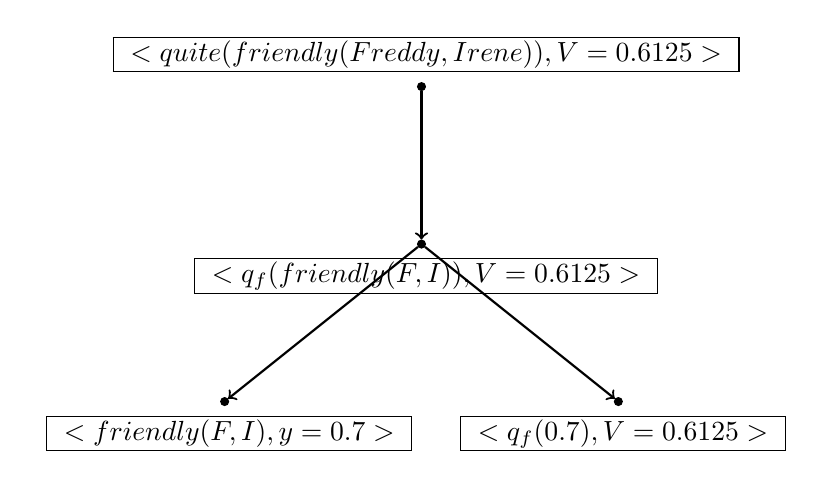
\begin{tikzpicture}[yscale=-1,
place/.style={circle,draw=black, fill=black, inner sep=0pt, 
              minimum size=1mm}]

\node[place] (1st) at (2.5, 0) [label=above: {
             \begin{tabular}{|c|}
               \hline
              	$<quite(friendly(Freddy,Irene)), V=0.6125>$\\
               \hline
             \end{tabular} }] {};

\node[place] (2nd) at (2.5, 2) [label=below: {
             \begin{tabular}{|c|}
               \hline
               $<q_{f}(friendly(F,I)),V=0.6125>$ \\
               \hline
             \end{tabular} }
] {};
        
	
\node[place] (3rd) at (0, 4) [label=below: {
              \begin{tabular}{|c|}
                \hline
                 $<friendly(F,I), y=0.7>$ \\
                \hline
              \end{tabular} }
] {};

        \node[place] (4th) at (5, 4) [label=below: {
              \begin{tabular}{|c|}
               \hline
              $<q_{f}(0.7), V=0.6125>$ \\
               \hline
              \end{tabular} }
] {}; 

\draw[->, thick] (1st) -- (2nd);
\draw[->, thick] (2nd) -- (3rd);
\draw[->, thick] (2nd) -- (4th);

\end{tikzpicture}
\end{center}
\caption{Example of evaluating $<quite(friendly(Freddy,Irene)),V>$}
\label{fig:QuiteFriendly}   
\end{figure}